\chapterA{Trabajar sobre un repositorio remoto de manera local}
\pagestyle{fancy}


Para modificar el código de la web tendremos dos opciones. Ninguna de ellas va a ser editarlo desde la propia web ya que es poco eficiente y tedioso.

Durante toda esta sección mostraré como hacer las acciones tanto con GitKraken como con GitHub Desktop.

Para explicar mejor todo, se hará referencia a dos figuras presentadas en el último apartado. (Figuras \ref{fig:cap_git} y \ref{fig:cap_git})

\section{Clonar el repositorio}

Clonar un repositorio significa bajar el código que hay en GitHub a nuestro PC.

\begin{figure}[ht]
    \begin{minipage}{0.4\linewidth}
        \centering
        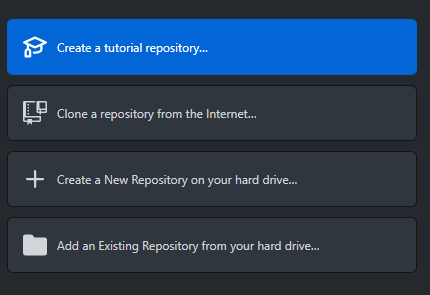
\includegraphics[width=0.9\linewidth,]{git_desk_vacio.png}
        \caption{Pantalla vacía de GitHub Desktop}
        \label{fig:cap_vacia}
    \end{minipage}%
    \begin{minipage}[b]{0.6\linewidth}
        \setlength{\parindent}{0.2in}

        Si vas a clonar un repositorio desde GitHub Desktop hay dos opciones: si no tienes más repositorios te saldrá como una opción en grande, en caso de tener más repositorios solo tienes que pulsar \textit{Ctrl + Shift + O}.

        Desde GitKraken solo tienes que pulsar \textit{Ctrl + N} para clonarlo.

        En ambos casos te pedirán que escojas el repositorio a clonar y donde clonarlo, la carpeta donde se descargará el código. En el caso de GitKraken tendrás que escoger GitHub como el proveedor.

    \end{minipage}
\end{figure}

\section{Subir código}

Parte importante de colaborar en un proyecto es modificar código y subir tus cambios.

Desde GitHub Desktop tendremos a la izquierda una pestaña con todos los archivos modificados (Figura \ref{fig:cap_git}: Cuadro 1). Al lado de estos archivos podemos marcar cuáles queremos subir y cuáles no.
Una vez escogidos cuáles subir pondremos una descripción (a poder ser más explicativa que \textit{Update file}) y le daremos al botón azul de \textit{Commit to main}. Tras esto solo falta irnos a la barra superior y darle a \textit{Push origin} (Figura \ref{fig:cap_git}: Cuadro 2). Esto último hará que subamos el código a GitHub y esté disponible para el resto del equipo.

En caso de usar GitKraken, las cosas son muy similares. A la izquierda tenemos una pestaña con los archivos modificados(Figura \ref{fig:cap_kraken}: Cuadro 1), tendremos que marcar uno por uno cuáles queremos subir dando click derecho al archivo y seleccionando \textit{Stage file}, en caso de querer seleccionarlos todos tendremos un botón verde que dirá \textit{Stage all changes}.
Tras esto pondremos una descripción y daremos al botón verde de \textit{Stage files to commit}. Solo falta ir a la barra de arriba y darle al botón de \textit{Push} (Figura \ref{fig:cap_kraken}: Cuadro 2)para subir los cambios al origen.

\section{Bajar cambios}

Antes de ponernos a picar código conviene mirar a ver qué han hecho nuestros compañeros en el tiempo en que no estábamos y bajarnos sus cambios.

En GitHub Desktop esto lo haremos desde la barra superior, en un botón en el que pondrá \textit{Fetch origin} (Figura \ref{fig:cap_git}: Cuadro 2). En caso de haber cambios el botón cambiará a \textit{Pull origin} (Figura \ref{fig:cap_git}: Cuadro 2). Si pulsamos esta vez nos bajará los cambios que haya en el repositorio.

En GitKraken se actualizará automáticamente en cierto intervalo de tiempo o al abrir la aplicación. Sabremos si hay algo nuevo porque en el gráfico saldrá un punto nuevo con una etiqueta ligeramente más oscura que la del gráfico principal. Una vez más para bajarnos el código solo tenemos que ir a la barra de arriba y pulsar en \textit{Pull} (Figura \ref{fig:cap_kraken}: Cuadro 3). En caso de que queramos actualizar los cambios y no se haya pasado el intervalo de tiempo, solo hay que ir al botón  de \textit{Pull}, darle a la flecha que hay al lado y seleccionar \textit{Fetch all}.

\section{Qué hacer cuando hay un \textit{commit} erróneo}

Todos cometemos errores, así que no está de más saber cómo arreglar un \textit{commit} que rompe el programa.

Aquí explicaremos un comando: \textit{git reset}.

El comando \textbf{reset} nos permite resetear, como bien indica su nombre, la cabeza del repositorio hasta un \textit{commit} anterior.
Esto se hará en tres posibles modos:
\begin{itemize}
    \item\textbf{Soft:} mueve la cabeza del repositorio al \textit{commit} seleccionado, pero no altera el repositorio. Los cambios entre el \textit{commit} y la antigua cabeza se quedarán confirmados para un nuevo \textit{commit}.
    \item\textbf{Mixed:} genera una copia de los datos posteriores al \textit{commit} al que se quiere volver.
    \item\textbf{Hard:} descarta todos los cambios posteriores al \textit{commit} deseado.
\end{itemize}

En GitKraken podremos seleccionar los modos dando click derecho a un commit y buscando la opción \textit{Reset main to this commit}.

GitHub Desktop y GitHub en su interfaz web no tienen, al momento de escribir esto, soporte para esta opción. La otra opción para hacer esto desde tu repositorio local sería hacerlo desde la línea de comandos.
